\subsection{Certified, excluded, and unresolved parameter regions}
\label{sec:region-diagnosis}
The three-way diagnostic separates sufficient coverage from demonstrated failure of the requested classifier family. Figure~\ref{fig:region-diagnosis} and Table~\ref{tab:region-diagnosis} report the original scaled endpoints at $K=100$ and penalty floor zero. At $t=s_C/8$, the sufficient certificate covers no queries, yet the combined witnesses exclude only 1.61\% of MNIST and 2.14\% of Fashion-MNIST queries. At $t=s_C$, the excluded proportions rise to 88.10\% and 84.48\%. The endpoint large-penalty witness alone accounts for 83.21\% and 66.27\%, respectively; narrower-width limit witnesses and archived finite predictions account for the remaining combined exclusions. Every certified/excluded intersection is empty.

\begin{figure}[!htbp]
\centering
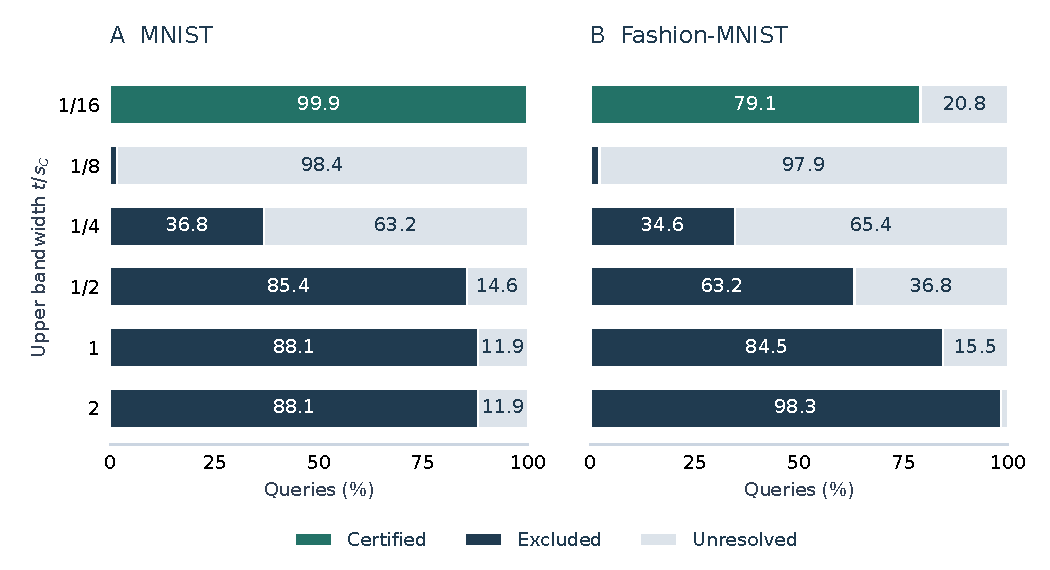
\includegraphics[width=\textwidth]{Figure_06_Agreement_Region_Diagnosis.pdf}
\caption{Three outcomes for the original regions $(0,t]\times[0,\infty)$ at $K=100$. Certified denotes the original sufficient condition; excluded denotes the union of guarded strict large-penalty and archived finite-score witnesses; unresolved denotes the remaining queries. Bars show five-seed mean percentages, with labels for segments of at least 10\%; Table~\ref{tab:region-diagnosis} gives exact rounded values and seed variation. The change from unresolved to excluded at broader endpoints distinguishes missing guarantees from identified failures of whole-region agreement.}
\label{fig:region-diagnosis}
\end{figure}

\begin{table}[!htbp]
\centering\small
\caption{Outcome partition at the original scaled widths, $K=100$ and $\lambda_0=0$. Entries are five-seed means $\pm$ sample standard deviations in percentage points; denominators are 4,027 MNIST or 10,000 Fashion-MNIST queries per seed.}
\label{tab:region-diagnosis}
\begin{tabular}{llrrr}
\toprule
Dataset & $t/s_C$ & Certified (\%) & Excluded (\%) & Unresolved (\%)\\
\midrule
MNIST & $1/16$ & 99.91 $\pm$ 0.06 & 0.06 $\pm$ 0.04 & 0.02 $\pm$ 0.03 \\
 & $1/8$ & 0.00 $\pm$ 0.00 & 1.61 $\pm$ 0.21 & 98.39 $\pm$ 0.21 \\
 & $1/4$ & 0.00 $\pm$ 0.00 & 36.76 $\pm$ 3.59 & 63.24 $\pm$ 3.59 \\
 & $1/2$ & 0.00 $\pm$ 0.00 & 85.40 $\pm$ 0.83 & 14.60 $\pm$ 0.83 \\
 & $1$ & 0.00 $\pm$ 0.00 & 88.10 $\pm$ 0.15 & 11.90 $\pm$ 0.15 \\
 & $2$ & 0.00 $\pm$ 0.00 & 88.13 $\pm$ 0.13 & 11.87 $\pm$ 0.13 \\
\midrule
Fashion-MNIST & $1/16$ & 79.09 $\pm$ 44.25 & 0.09 $\pm$ 0.03 & 20.82 $\pm$ 44.23 \\
 & $1/8$ & 0.00 $\pm$ 0.00 & 2.14 $\pm$ 0.98 & 97.86 $\pm$ 0.98 \\
 & $1/4$ & 0.00 $\pm$ 0.00 & 34.57 $\pm$ 4.41 & 65.43 $\pm$ 4.41 \\
 & $1/2$ & 0.00 $\pm$ 0.00 & 63.23 $\pm$ 2.74 & 36.77 $\pm$ 2.74 \\
 & $1$ & 0.00 $\pm$ 0.00 & 84.48 $\pm$ 4.98 & 15.52 $\pm$ 4.98 \\
 & $2$ & 0.00 $\pm$ 0.00 & 98.32 $\pm$ 3.21 & 1.68 $\pm$ 3.21 \\
\bottomrule
\end{tabular}
\end{table}

The dense grid resolves the loss of sufficient coverage more precisely. For each seed, we inspect the first grid width after the largest width retaining any sharp certification. At floor zero, the mean upper widths are $0.09622s_C$ for MNIST and $0.08638s_C$ for Fashion-MNIST. The excluded proportions are only $0.38\pm0.15$\% and $0.44\pm0.32$\%, leaving 99.62\% and 99.56\% unresolved. These measurements place the sufficient frontier and the demonstrated broad-width obstruction in distinct regimes. The tests identify extensive failures farther into the bandwidth range and leave the immediate sufficient frontier open to tighter analysis.

\subsection{Local bandwidth bands with finite penalty thresholds}
\label{sec:tail-results}
Theorem~\ref{thm:local-tail} certifies positive local bandwidth bands at both broader endpoints. Table~\ref{tab:local-tail} reports $[0.99t,t]\times[10\norm{A_t}_2,\infty)$. At $t=s_C/2$, the signed interval condition covers 16.88\% of MNIST and 40.09\% of Fashion-MNIST queries. At $t=s_C$, it covers 16.79\% and 14.94\%. Retaining signs in the correction term materially changes coverage: at $t=s_C$, the positive-sum comparator covers 2.34\% of MNIST and no Fashion-MNIST queries at the same penalty floor. Among queries with positive interval margins, the mean within-seed median signed thresholds are $1.18\norm{A_t}_2$ and $1.38\norm{A_t}_2$ at $t=s_C/2$, and $1.14\norm{A_t}_2$ and $2.35\norm{A_t}_2$ at $t=s_C$.

\begin{table}[!htbp]
\centering\small
\caption{Local-band certification and fitted accuracy for $s=0.99t$ and penalty floor $\Lambda=10\norm{A_t}_2$, at $K=100$. Coverage refers to the full continuous band and tail; accuracy evaluates the fitted endpoint $(t,\Lambda)$ against dataset labels. Entries are five-seed means $\pm$ sample standard deviations in percentage points.}
\label{tab:local-tail}
\begin{tabular}{llrrr}
\toprule
 & & \multicolumn{2}{c}{Certified coverage (\%)} & Readout\\
Dataset & $t/s_C$ & Positive-sum & Signed interval & accuracy (\%)\\
\midrule
MNIST & $1/2$ & 16.79 $\pm$ 1.19 & 16.88 $\pm$ 1.13 & 15.60 $\pm$ 1.35 \\
 & $1$ & 2.34 $\pm$ 3.71 & 16.79 $\pm$ 1.19 & 11.77 $\pm$ 0.00 \\
\midrule
Fashion-MNIST & $1/2$ & 23.94 $\pm$ 5.22 & 40.09 $\pm$ 4.95 & 45.06 $\pm$ 2.57 \\
 & $1$ & 0.00 $\pm$ 0.00 & 14.94 $\pm$ 2.28 & 29.86 $\pm$ 6.34 \\
\bottomrule
\end{tabular}
\end{table}

Increasing the relative bandwidth span to $[0.95t,t]$ retains signed coverage of 16.77\% and 22.15\% at $t=s_C/2$ for MNIST and Fashion-MNIST, respectively. At $t=s_C$, coverage is 16.78\% for MNIST and zero for Fashion-MNIST. The interval-margin condition itself fails for every Fashion-MNIST query in that last setting. This sensitivity shows how the local width interval enters the guarantee.

Across the 120 newly fitted readouts, all 254,120 certified query--parameter checks agree with the nearest-prototype label. The corresponding all-query endpoint accuracies at $10\norm{A_t}_2$ are 15.60\% and 45.06\% at $t=s_C/2$, and 11.77\% and 29.86\% at $t=s_C$, for MNIST and Fashion-MNIST respectively. Section~\ref{sec:r3-selectors} evaluates the certified-subset accuracies against matched-coverage selectors and reports the selected class distributions. The new regions establish computable label agreement at broader widths and identify its penalty-dependent accuracy tradeoff.
